\documentclass[draft]{fhnwreport}         %[mode] = draft or final
%%---Main Packages-----------------------------------------------------------------------
\usepackage[english, ngerman]{babel}	%Mul­tilin­gual sup­port for LaTeX
\usepackage[T1]{fontenc}				      %Stan­dard pack­age for se­lect­ing font en­cod­ings
\usepackage[utf8]{inputenc}				  %Ac­cept dif­fer­ent in­put en­cod­ings
\usepackage{lmodern}                 %The newer Font-Set
\usepackage{textcomp}					      %LaTeX sup­port for the Text Com­pan­ion fonts
\usepackage{graphicx} 					      %En­hanced sup­port for graph­ics
\usepackage{float}						        %Im­proved in­ter­face for float­ing ob­jects
%\usepackage{ifdraft}                %Let you check if the doc is in draft mode

%%---Useful Packages---------------------------------------------------------------------
%\usepackage[pdftex,dvipsnames,tables]{xcolor}  %Driver-in­de­pen­dent color ex­ten­sions for LaTeX
\usepackage[table,xcdraw]{xcolor}
\usepackage{csquotes}                %Simpler quoting with \enquote{}
\usepackage{siunitx} 					      %A com­pre­hen­sive (SI) units pack­age
\usepackage{listings}					      %Type­set source code list­ings us­ing LaTeX
\usepackage[bottom]{footmisc}			  %A range of foot­note op­tions
\usepackage{footnote}					      %Im­prove on LaTeX's foot­note han­dling
\usepackage{verbatim}					      %Reim­ple­men­ta­tion of and ex­ten­sions to LaTeX ver­ba­tim
\usepackage[textsize=footnotesize]{todonotes} %Mark­ing things to do in a LaTeX doc­u­ment
\usepackage{lipsum}              % Gives you access to blindtext

%%---Tikz Packages-----------------------------------------------------------------------
%\usepackage{standalone}
%\usepackage{tikz}
%\usepackage{circuitikz}
%\usetikzlibrary{arrows}
%\usetikzlibrary{calc}
%\usetikzlibrary{intersections}

%%---Math Packages-----------------------------------------------------------------------
\usepackage{amsmath}					    %AMS math­e­mat­i­cal fa­cil­i­ties for LaTeX
%\usepackage{amssymb}					  %Type­set­ting symbols (AMS style)
%\usepackage{array}						  %Ex­tend­ing the ar­ray and tab­u­lar en­vi­ron­ments
%\usepackage{amsthm}					    %Type­set­ting the­o­rems (AMS style)

%%---Table Packages----------------------------------------------------------------------
\usepackage{tabularx}					  %Tab­u­lars with ad­justable-width columns
%\usepackage{longtable}
\usepackage{multirow}					  %Create tab­u­lar cells span­ning mul­ti­ple rows
\usepackage{multicol}					  %In­ter­mix sin­gle and mul­ti­ple columns
\usepackage{graphicx}
\usepackage{colortbl}

%%---PDF / Figure Packages---------------------------------------------------------------
\usepackage{pdfpages}					  %In­clude PDF doc­u­ments in LaTeX
\usepackage{pdflscape}					  %Make land­scape pages dis­play as land­scape
%\usepackage{subfig}					    %Fig­ures di­vided into sub­fig­ures
\usepackage{eforms}

%%---Other Packages----------------------------------------------------------------------
%\usepackage{xargs}              %De­fine com­mands with many op­tional ar­gu­ments


%%---Main Settings-----------------------------------------------------------------------
\graphicspath{{./graphics/}}			%Defines the graphicspath
%\geometry{twoside=false}				%twoside=false disables the "bookstyle"
\setlength{\marginparwidth}{2cm}
\overfullrule=5em						    %Creates a black rule if text goes over the margins => debugging

%%---User Definitions--------------------------------------------------------------------
%%Tabel-Definitions: (requires \usepackage{tabularx})
\newcolumntype{L}[1]{>{\raggedright\arraybackslash}p{#1}}    %column-width and alignment
\newcolumntype{C}[1]{>{\centering\arraybackslash}p{#1}}
\newcolumntype{R}[1]{>{\raggedleft\arraybackslash}p{#1}}					                        %loads all packages, definitions and settings	

%%%%% Bibliographie entweder im IEEE- oder im APA-Stil:
%\usepackage[style=ieee,urldate=comp,backend=biber]{biblatex}
\usepackage[style=apa,urldate=comp,backend=biber]{biblatex}
%%%%%
\addbibresource{literature/beispiel_bib.bib}
											
\title{Autonomous Beer-Cooler}  %Project Title
\author{Semesterarbeit}    %Document Type => Technical Report, ...
\date{Muttenz, Januar 2023}               %Place and Date

\begin{document}

\pagenumbering{roman}	

%%---TITLEPAGE---------------------------------------------------------------------------
\selectlanguage{ngerman}                  %ngerman or english
\maketitle

\vfill

\begin{figure}[H]
\centering

\includegraphics[width=4cm]{knauber.jpg}
\end{figure}

\vfill

\begin{tabular}{@{}p{5cm} l}
Studenten          &    Max Knauber\\
                           &    Matthias Gass\\
                           &    Fabian Schenker\\[2ex]
Fachbetreuer            &    Silvan Wirth\\[2ex]
\multicolumn{2}{@{}l}{Fachhochschule Nordwestschweiz, Hochschule für Technik}
\end{tabular}

\vspace*{4ex}
% Logo
\begin{tikzpicture}[remember picture,overlay,every node/.style={anchor=north west}]
  \node at (current page.north west) [xshift=0.5cm, yshift=-0.5cm] {
\includegraphics[width=20cm]{logo_neu.pdf}};
\end{tikzpicture}

\clearpage
			
%%---ABSTRACT-------------------------------------------------------------------
\selectlanguage{ngerman}				%ngerman or english
\thispagestyle{empty}
\include{sections/00_zusammenfassung}
\section*{Vorwort / Dank}
\addcontentsline{toc}{section}{Vorwort / Dank}

Dieses Projekt hat gezeigt, wie wichtig eine gute Zusammenarbeit und Einsatz der fachlichen und sozialen Kompetenzen von jedem ist, die zum Erfolg von diesem Projekt beigetragen haban. \\
\\
Der FHNW danken wir für die Arbeitsmöglichkeiten im Labor, der Werkstatt und den Gruppenräumen.\\
\\
Herrn Silvan Wirth danken wir für die Begleitung während des Projekts und für die Beantwortung bei allfälligen Fragen.\\
\\
Wir danken uns gegenseitig für die gute Zusammenarbeit.\\
\\
Weiter geht unser Dank an alle weiteren Personen, welche hier nicht namentlich aufgelistet sind und uns bei dieser Projektarbeit ebenfalls unterstützt haben.

\section*{Rahmenbedingungen}
\addcontentsline{toc}{section}{Rahmenbedingungen}

\subsection*{Übersicht}
\begin{itemize}
    \item Zu realisierende Projekte können vorgeschlagen werden (Berücksichtigung gewisser Rahmenbedingungen)
    \item Bearbeitung in Zweier- oder Dreiergruppen
    \item Vorgabe SGL: lauffähige Produkte mit Aussenwirkung für Marketing
    \item Zuweisung von max. zwei Gruppen auf ein Projekt
    \item Austausch zwischen Gruppen möglich (Lösungsvarianz höher, Chance, dass ein lauffähiges Produkt entsteht, ist höher)
\end{itemize}
 

\subsection*{Rahmenbedingungen Projekte}
\begin{itemize}
    \item Enthält Merkmale eines mechatronischen Systems (Sensorik, Aktorik, Informationsverarbeitung (Rechner / Steuerung))
    \item Aktorik: physische Bewegung muss vorhanden sein
    \item User-Interface: optional, nicht zwingend
    \item Energieversorgung sinnvoll gelöst    
\end{itemize}

\subsection*{Qualifikationsziele und Kompetenzen}
\begin{itemize}
    \item Sachkompetenz:
    \begin{itemize}
        \item Verstehen und praktisches Anwenden der mechatronischen Modellbildung
    \end{itemize}
    \item Selbstkompetenz:
    \item \begin{itemize}
        \item Eigenständige Auswahl und Einsatz von Aktoren, Sensoren, Mikrorechner
    \end{itemize}
    \item Sozial-ethische Kompetenz:
    \begin{itemize}
        \item ein System vom Konzept bis zum funktionierenden Produkt entwickeln.
        \item mechatronisches Projekt im Team erfolgreich planen und durchführen.
        \item gruppendynamische Prozesse bei der Bearbeitung größerer Aufgaben innerhalb von Projektgruppen erfahren
    \end{itemize}
\end{itemize}

\subsection*{Unterstützung des Lernprozesses}
\begin{itemize}
    \item Aufwand gemäss Modulhandbuch: 15 h Präsenz, 45 h Selbststudium
    \item Anwenden des theoretischen Wissens aus der Vorlesung «Mechatronische Systeme» (und aller anderer vorgängiger Vorlesungen)
    \item Praktische Realisierung wird begleitet durch Dozenten.    
\end{itemize}

\subsection*{Verknüpfung in Modulgruppe Mechatronik III}
\begin{itemize}
    \item Fach «Mechatronische Systeme» wirkt auf Fach «Mechatronisches Labor»
    \item Inhalte und Methoden aus Vorlesung sollen angewendet werden
    \item Unterstützung bei Realisierung eines konkreten Projektes
\end{itemize}

\subsection*{Prüfungsbedingungen}
\begin{itemize}
    \item Leistungserfassung durch Präsentation und Bewertung des Projektes
    \item Termin: 10.01.2023	08:30 – 12:15
    \item Gewichtung: Schlussnote gemäss Bewertungsraster
\end{itemize}

\subsection*{Youtube-Videos / Mechatronik-Trinational Channel}
Zu den Projekten werden Videos gestaltet. Diese fliessen in die Bewertung der Projekte mit ein (siehe Bewertungsraster).\\
\\
Das Video Ihres Projektes muss «Youtube-konform» sein, z.B. sind die Musik-Copyrights zu beachten und wenn Sie (aus welchen Gründen auch immer) nicht im Video zu sehen sein wollen, dann sollten Sie sich auch nicht selbst aufnehmen.

\subsection*{Projektrahmen}
\begin{itemize}
    \item Kostendeckel CHF 200.-pro Projekt
    \item Kann ggf. bei marketingtechnischem Nutzen erhöht werden (nach vorheriger Absprache)
    \item Materialbeschaffung selbst zu organisieren
    \item Abrechnung über Sekretariat/Studiengangsleitung zum Ende des Semesters    
    \item Aufstellung mit Belegen und Kontoverbindung (IBAN) gemäss Formular
    \item Projekt muss vorgängig durch Dozenten genehmigt werden
    \item Arduino und/oder RaspberryPi wird abgegeben durch Labor (muss nicht in den Projektkosten berücksichtigt werden)
\end{itemize}

\subsection*{Laborzugang und Werkstattbenutzung}
\begin{itemize}
    \item Die Studierenden dürfen aus Sicherheits-und Versicherungsgründen das Labor Mechatronik Trinational / Campus Muttenz nicht unbegleitet (ohne Dozierenden) nutzen
    \item Zugang Labor Mechatronik Trinational gem. Unterrichtszeiten
    \item Werkstattaufträge (extern oder Hochschulen) sind vorgängig mit dem Dozierenden abzusprechen
    \item Kosten sind vorgängig zu klären und fliessen ins Projektbudget ein 
\end{itemize}

%%---TABLE OF CONTENTS-----------------------------------------------------------	
\selectlanguage{ngerman}				%ngerman or english
\tableofcontents
\clearpage

\listoffigures
\listoftables
\cleardoublepage

%%---TEXT--------------------------------------------------------------------
\pagenumbering{arabic}
\section{Einleitung}

\lipsum[6-7]

\section{Vorstudie}

\subsection{Systemabgrenzung}

Anlässlich des anstehenden Projekts für das fünfte Semester möchten wir uns 
hier mit der Vorstudie befassen. Die Systemabgrenzung, angefangen nach den Umfeld
nach PESTEL-Guidelines (Abbildung~\ref{fig:pestel}) zeigt an sich weder Details 
noch Unerwartetes.

\begin{figure}[h]
\begin{center}
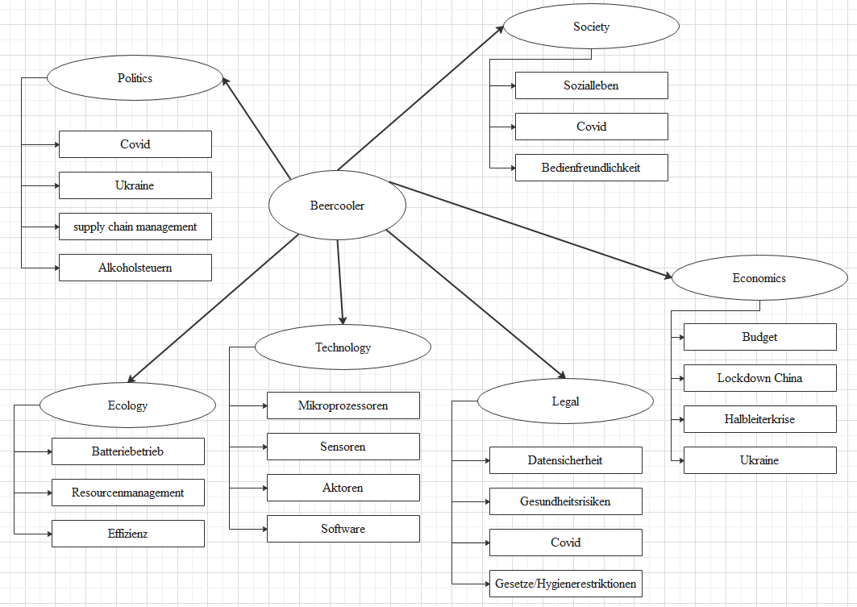
\includegraphics[width=\linewidth]{graphics/pestel.png}
\end{center}
\caption{Umfeld der Systemabgrenzung nach PESTEL}
\label{fig:pestel}
\end{figure}

\pagebreak

Das Eingriff System (Abbildung~\ref{fig:systemabgrenzung}) mit Umsystem hingegen 
vermittelt bereits ein deutlich klareres Bild.

\begin{figure}[h]
\begin{center}
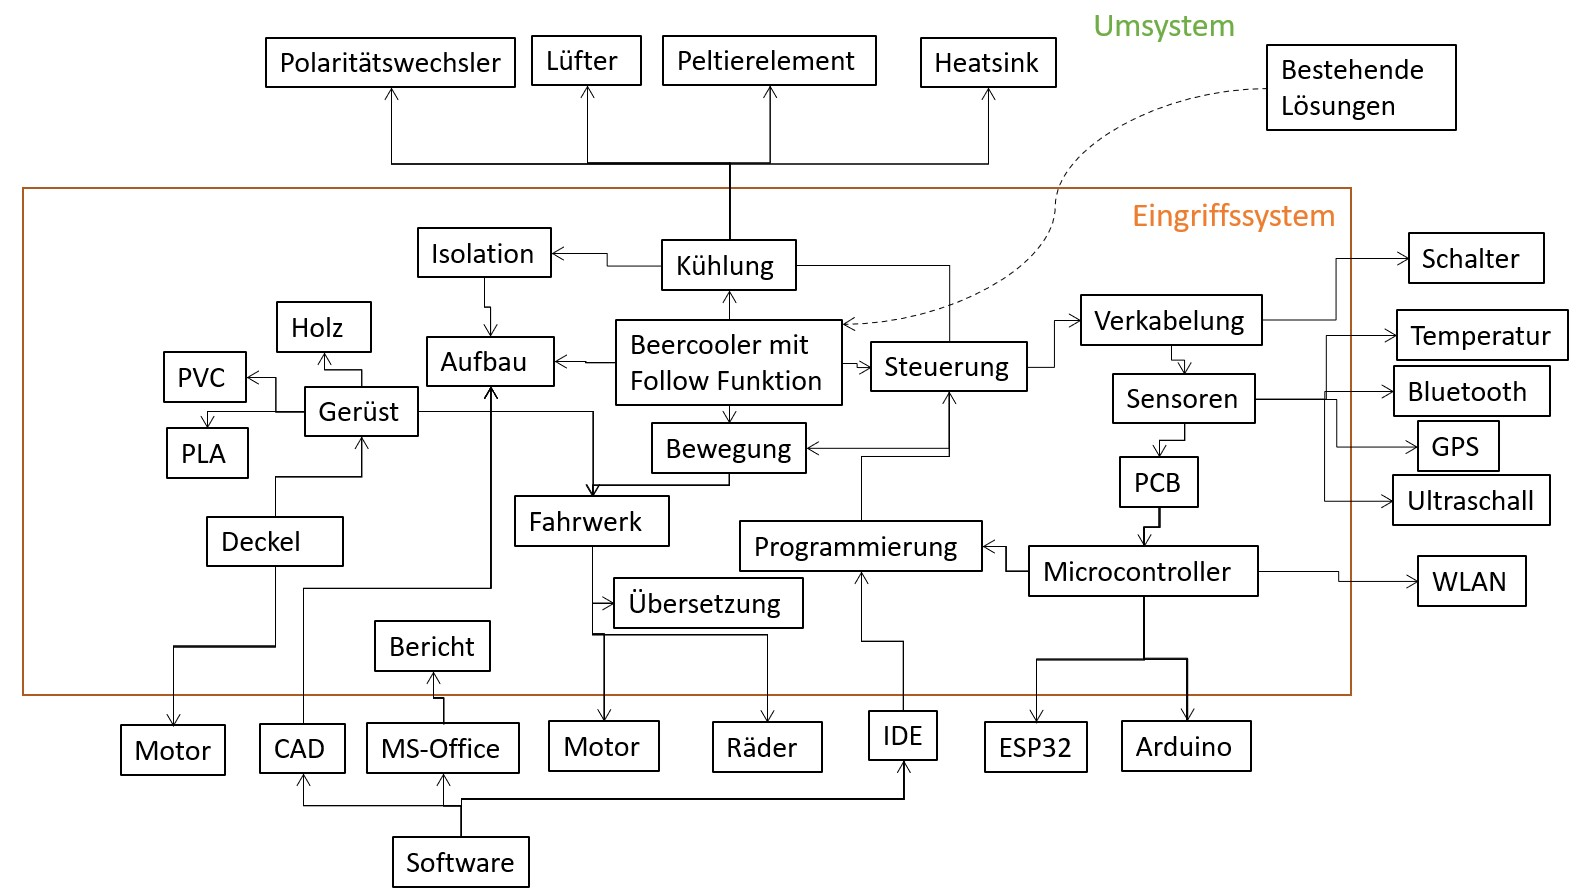
\includegraphics[width=\linewidth]{graphics/systemabgrenzung.jpg}
\end{center}
\caption{Umfeld der Systemabgrenzung nach PESTEL}
\label{fig:systemabgrenzung}
\end{figure}

\subsection{Zielkatalog}

Der Zielkatalog beschreibt unsere Anforderungen an das Projekt. Level 1 sind 
hierbei Ziele, die unbedingt erfüllt sein müssen, während Level 2 und 3 
Ausbaustufen darstellen, die weniger stark priorisiert werden. Zusammengefasst 
soll der Roboter also in der Lage sein, autonom einer Person zu folgen, 
mindestens ein Dutzend Bier zu beinhalten und diese über eine gewisse Zeit 
aktiv zu kühlen.

\textbf{Zielkatalog Level 1}



\textbf{Zielkatalog Level 2}



\textbf{Zielkatalog Level 3}


\section{Kapitel This}

\lipsum[9]

\subsection{Untertitel 1}

\lipsum[10]

\subsection{Untertitel 2}

\lipsum[11]

\subsubsection{Untertitel 3.~Grades}

Tabelle~\ref{tab:beispieltabelle} zeigt etwas. \lipsum[14-14]

\begin{table}
  \begin{center}
    \renewcommand{\arraystretch}{1.2}
    \begin{tabular}{l|S|S}\hline
      Medium & {Dichte $\rho$ in \SI{}{\kilogram\per\cubic\meter}} & 
               {Schallgeschwindigkeit $c$ in \SI{}{\meter\per\second}}\\
      \hline
		Luft \SI{0}{\degree C} trocken & 1.293 & 331 \\
		Wasserstoff \SI{0}{\degree C} & 0.090 & 1260 \\
		Wasser \SI{0}{\degree C} & 1000 & 1400 \\
		Holz & 600 & 4500 \\
		Stahl & 7700 & 5050 \\
		\hline
    \end{tabular}
  \end{center}
  \caption[Schallgeschwindigkeit in verschiedenen Medien]{Schallgeschwindigkeit in verschiedenen Medien gemäss \cite[S.~566]{hering_physik_2016}}
  \label{tab:beispieltabelle}
\end{table}

\lipsum[15-15]

\subsubsection{Untertitel 3.~Grades}

\lipsum[16-17]
\section{Kapitel That}

\lipsum[42]

\subsection{Code-Beispiel}

\lipsum[43]

\lstdefinestyle{custompython}{
  belowcaptionskip=1\baselineskip,
  breaklines=true,
  frame=L,
  xleftmargin=\parindent,
  numbers=left,
  language=Python,
  showstringspaces=false,
  basicstyle=\footnotesize\ttfamily,
  keywordstyle=\bfseries\color{green!40!black},
  commentstyle=\itshape\color{purple!40!black},
  identifierstyle=\color{blue},
  stringstyle=\color{orange},
}

\lstinputlisting[caption=Ein kurzes Codebeispiel in der Programmiersprache Python, style=custompython]{listings/python_example.py}

\section{Schlussbemerkungen}

\lipsum[28]


%%---BIBLIOGRAPHY-------------------------------------------------------
{\sloppypar
\printbibliography[heading=bibintoc, title=Quellenverzeichnis]
}

%%---APPENDIX----------------------------------------------------------
\section*{Ehrlichkeitserklärung}
\addcontentsline{toc}{section}{Ehrlichkeitserklärung}

Hiermit erkläre ich, die vorliegende [Projektarbeit, Individualarbeit, Bachelorarbeit etc.] selbständig und nur unter Benutzung der angegebenen Quellen verfasst zu haben. Die wörtlich oder inhaltlich aus den aufgeführten Quellen entnommenen Stellen sind in der Arbeit als Zitat bzw. Paraphrase kenntlich gemacht. Diese [Studien-/Projektarbeit/Bachelor Thesis] ist noch nicht veröffentlicht worden. Sie ist somit weder anderen Interessierten zugänglich gemacht noch einer anderen Prüfungsbehörde vorgelegt worden.

\vspace*{4ex}

Windisch, tt. Monat 20jj

\vspace*{4ex}

{\renewcommand{\arraystretch}{2}
\begin{tabular}{@{}>{\bf}ll}
Name: & Pia Musterfrau\\
Unterschrift: & \\[6ex]
Name: & Michael Mustermann\\
Unterschrift: & \\
\end{tabular}
\begin{appendix} %Anhang

\listoffigures
\listoftables

\pagebreak

\section{Anhang / Ressourcen}

\subsection{Impressum}
Datum der Erstellung der Dokumentation: Herbst und Winter 2022/2023\\
\\
© Fachhochschule Nordwestschweiz, Studiengang Mechatronik Trinational, 2023

\subsection{Quellcode}

\lstinputlisting[language=C++,frame=single,label=coolercode,caption=Programm des Roboters]{code/Cooler_FaMaMa.ino}
\lstinputlisting[frame=single,label=coolerdefinition,caption=Definitionen für das Programm]{code/CoolerDefinitions.h}

\end{appendix}


%%---NOTES for DEBUG---------------------------------------------------------------------
%\newpage
%\listoftodos[\section{Todo-Notes}]
%\clearpage

\end{document}